\documentclass{article}

\usepackage[utf8]{inputenc}
\usepackage[T1]{fontenc}
\usepackage[greek,english]{babel}
\usepackage{alphabeta}
\usepackage{amsmath}
\usepackage{amssymb}
\usepackage{graphicx}
\usepackage{subcaption}
\usepackage{epstopdf}
\usepackage[margin=1in, paperwidth=8.3in,paperheight=11.7in]{geometry}
\usepackage{hyperref}
\usepackage{paracol}

\newcommand\course{ΗΡΥ 411}
\newcommand\courseName{Ενσωματωμένα Συστήματα Μικροεπεξεργατών}
\newcommand\semester{Χειμερινό 2020-2021}
\newcommand\assignmentNumber{Εργαστήριο 10}
\newcommand\studentName{Μαυρογιώργης Δημήτρης}                           
\newcommand\studentNumber{2016030016}

\title{\underline{\textbf{\assignmentNumber}}} 
\author{\textsc{\textbf{Όνομα:}}  \studentName\\
		\textsc{\textbf{ΑΜ:}}  \studentNumber\\
		\course \ - \courseName\\ 
		\textsc{Πολυτεχνείο Κρήτης}
		}
\date{\today}
\begin{document}
	\maketitle

\section*{Σκοπός}
	Σκοπός του δέκατου εργαστηρίου είναι να κατανοήσουμε τις υπολογιστικές δυνατότητες ενός μικροελεγκτή AVR κάνοντας ένα απλό πρόγραμμα πολλαπλασιασμού πινάκων 3x3 με δύο δυαφορετικού τρόπους: 1) χρησιμοποιώντας ως τύπο δεδομένων integers και 2) χρησιμοποιώντας ως τύπο δεδομένων floats. 

\section*{Περιγραφή της υλοποίησης}
	Αρχικά, δηλώθηκαν 6 arrays, εκ των οποίων τα 3 είναι τύπου int και τα άλλα 3 είναι τύποθ float. Πιο συγκεκριμένα για κάθε τύπο δεδομένων έχουμε τους 2 πίνακες που πολλαπλασιάζουμε και έναν τρίτο στο οποίο αποθηκεύουμε το αποτέλεσμα. Ολα τα δεδομένα των πινάκων, καθώς και τα αποτελέσματα του πολλαπλασιασμού βρίσκονται στημνήμη του AVR. \\
	
	\noindent
	H αρχικοποίηση των πινάκων που πολλαπλασιάζουμε γίνεται κατά τη δήλωση των global arrays. Επιπλέον για τον πολλαπλασιασμό των πινάκων δημιουργήθηκαν δύο ίδιες ρουτίνες με μοναδική διαφορά ότι η πρώτη κάνει το πολλαπλασιασμό των int arrays, ενώ η δεύτερη κάνει τον πολλαπλασισμό των float arrays. H υλοποίησή τους είναι απλή και με ένα τριπλό βρόγχο επανάληψης υπολογίζουμε μέσω πολλαπλασιασμών και προσθέσεων το κάθε στοιχείο του τελικού πίνακα.\\
	
	\noindent
	Τέλος, όσον αφορά τη main, έχουμε το iddle loop, ενώ καλούμε τις δύο συναρτήσεις για τον πολλαπλασιασμό των πινάκων.
	
	\begin{figure}[h!]
		\centering
		\begin{subfigure}[t]{0.5\textwidth}
			\centering
			\includegraphics[height=3.5cm, width=\linewidth]{./results/lab10_defineS.png}
			\caption{C code for defines}
		\end{subfigure}%
		~
		\begin{subfigure}[t]{0.5\textwidth}
			\centering
			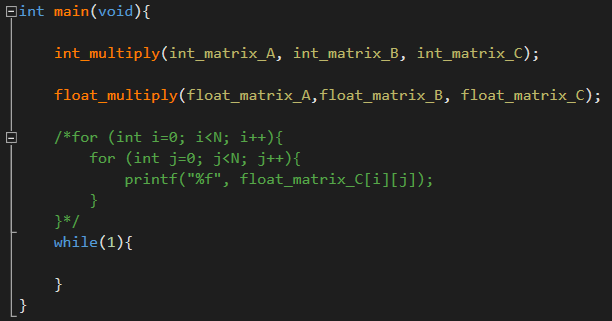
\includegraphics[height=3.5cm, width=\linewidth]{./results/lab10_main.png}
			\caption{C code for main}
		\end{subfigure}
	
		\begin{subfigure}[t]{0.5\textwidth}
			\centering
			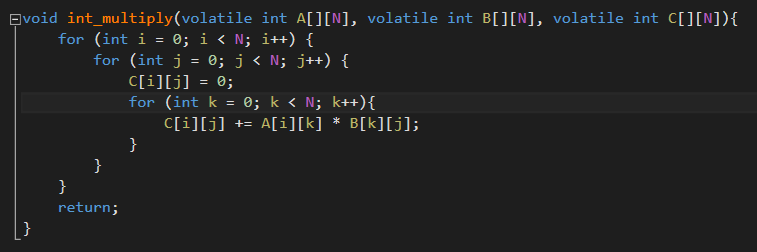
\includegraphics[height=3.5cm, width=\linewidth]{./results/lab10_int_multiplication.png}
			\caption{C code for INT multiplication function}
		\end{subfigure}%
		~
		\begin{subfigure}[t]{0.5\textwidth}
			\centering
			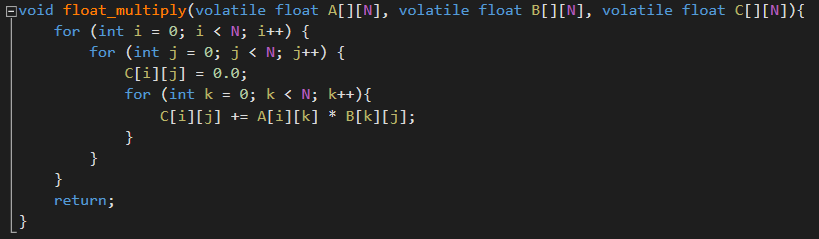
\includegraphics[height=3.5cm, width=\linewidth]{./results/lab10_float_multiplication.png}
			\caption{C code for FLOAT multiplication function}
		\end{subfigure}
	\end{figure}
	
	\pagebreak
	\noindent
	\textbf{Προσομοίωση Αποτελεσμάτων} \\
	
	\noindent
	Όπως παρατηρούμε και στις δύο προσομοιώσεις για integers και floats, ο κάθε αριθμός που αποθηκεύουμε καταλαμβάνει χώρο στη μνήμη ίσο με 4 bytes. Συνεπώς, για την αποθήκευση ενός πίνακα 3x3 χρειαζόμαστε χώρο 36 bytes, καθώς αποθηκεύουμε 9 αριθμούς για κάθε πίνακα.	Επιπλέον, βλέπουμε ότι η ρουτίνα για τον υπολογισμό του γινομένου των 2 integer πινάκων χρειάζεται 2824 - 1337 = 1487 κύκλους. \\
	\begin{figure}[h!]
		\centering
		\begin{subfigure}[t]{0.5\textwidth}
			\centering
			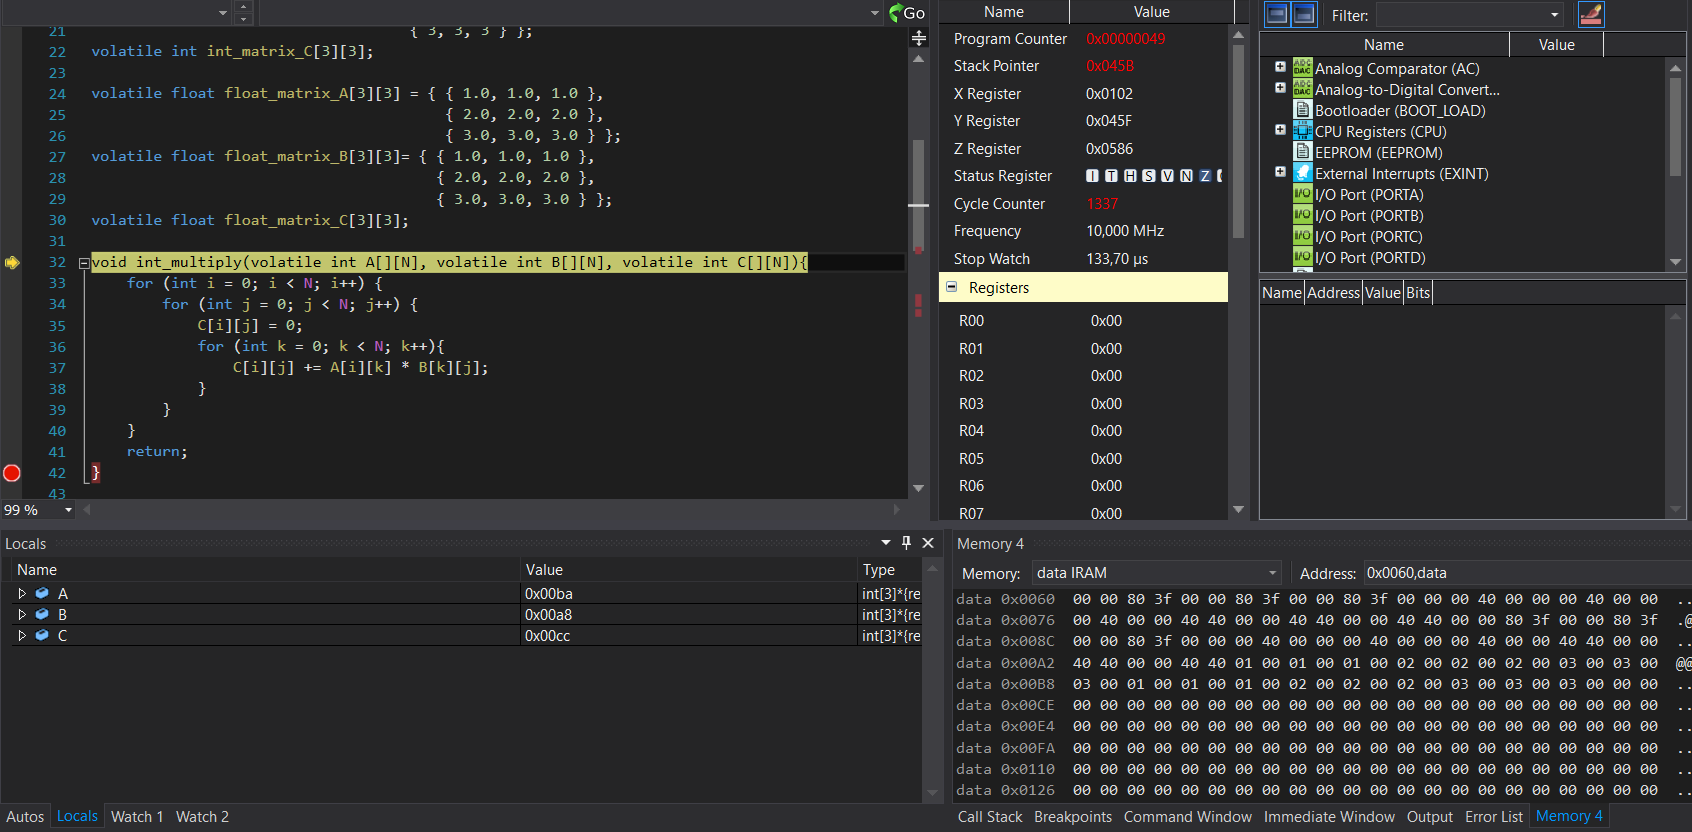
\includegraphics[height=3.5cm, width=\linewidth]{./results/lab10_sim_ints_a.png}
		\end{subfigure}%
		~
		\begin{subfigure}[t]{0.5\textwidth}
			\centering
			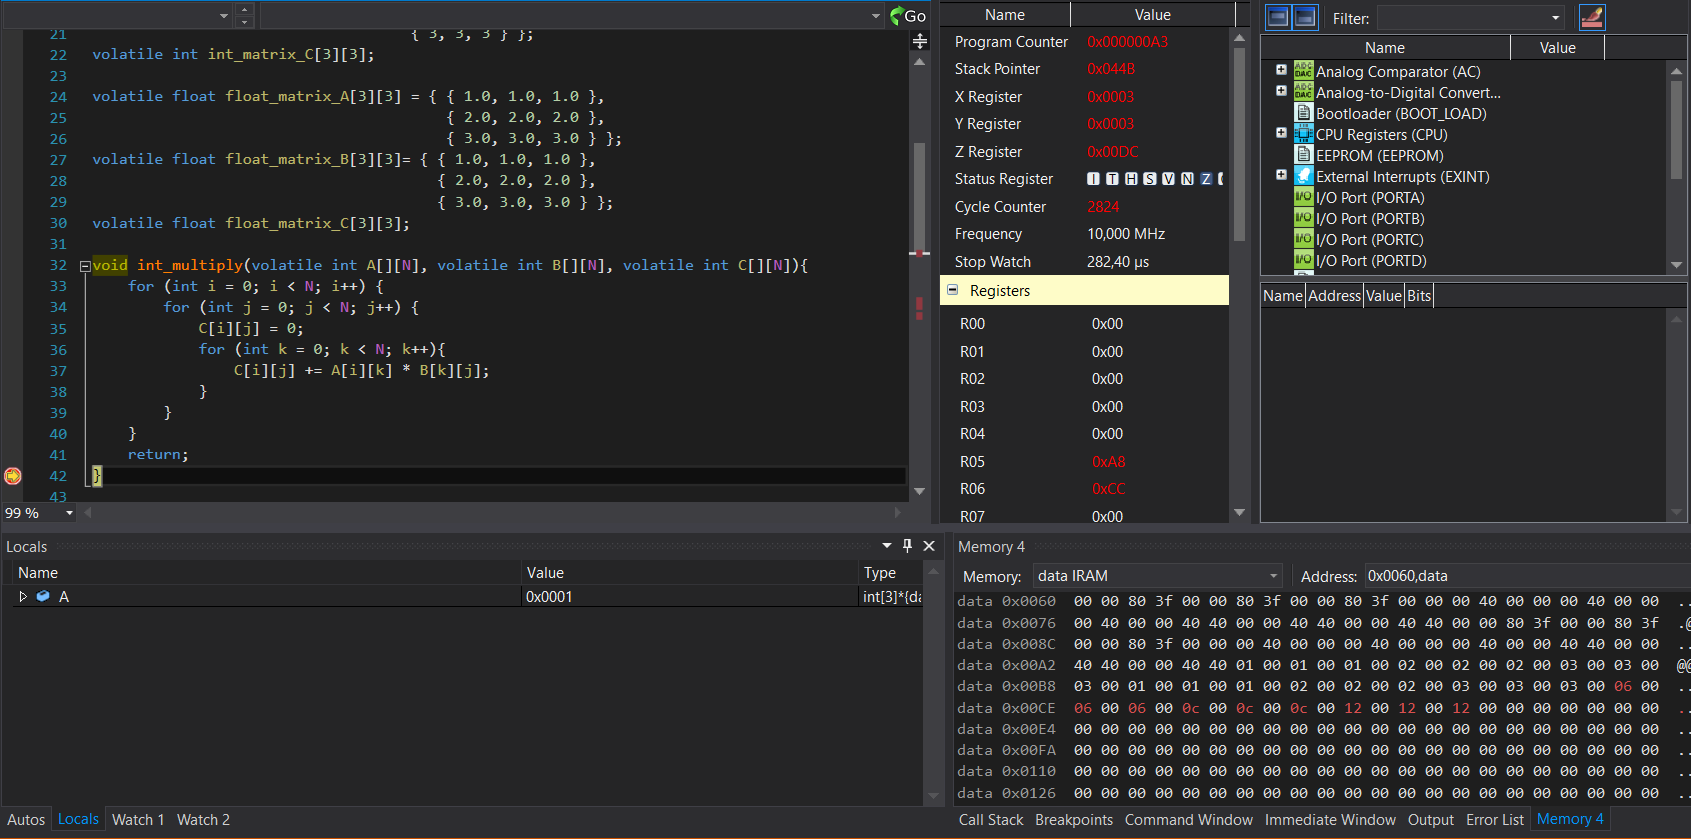
\includegraphics[height=3.5cm, width=\linewidth]{./results/lab10_sim_ints_b.png}
		\end{subfigure}
		\caption{Results from Αtmel Studio 7 - INT multiplication}
	\end{figure}

	\noindent
	Όσον αφορά τον υπολογισμό του γινομένου float αριθμών ο ίδιος αλγόριθμος όταν εντελεστεί από το μικροελεγκτή AVR, για να υπολογίσει το αποτέλεσμα χρειάζεται 11040 - 2870 = 8170 κύκλους.\\
	\begin{figure}[h!]
		\centering
		\begin{subfigure}[t]{0.5\textwidth}
			\centering
			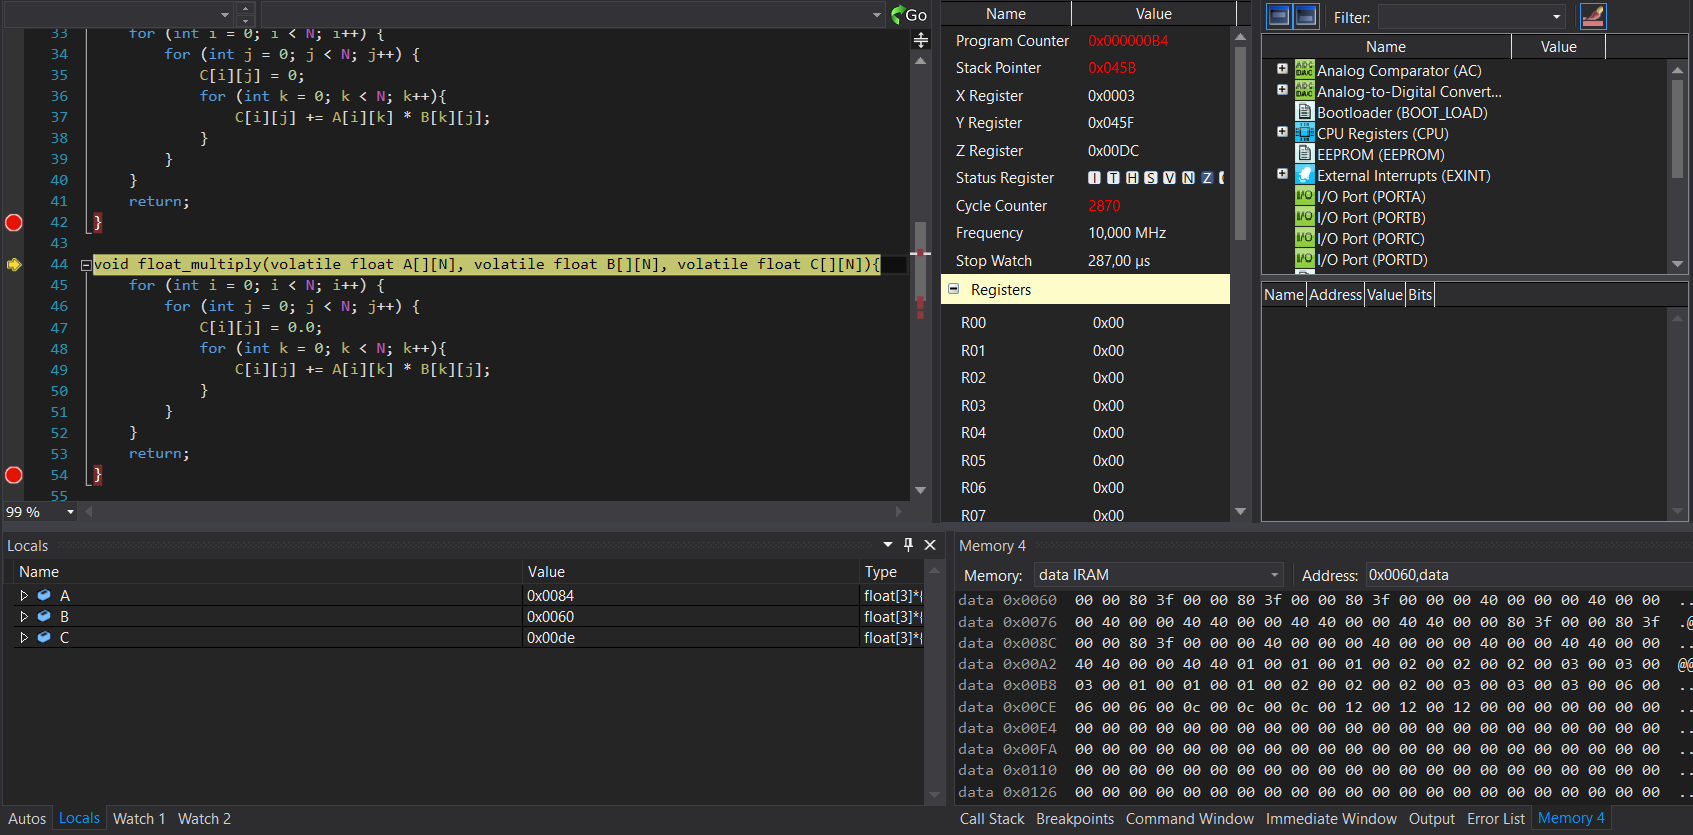
\includegraphics[height=3.5cm, width=\linewidth]{./results/lab10_sim_floats_a.png}
		\end{subfigure}%
		~
		\begin{subfigure}[t]{0.5\textwidth}
			\centering
			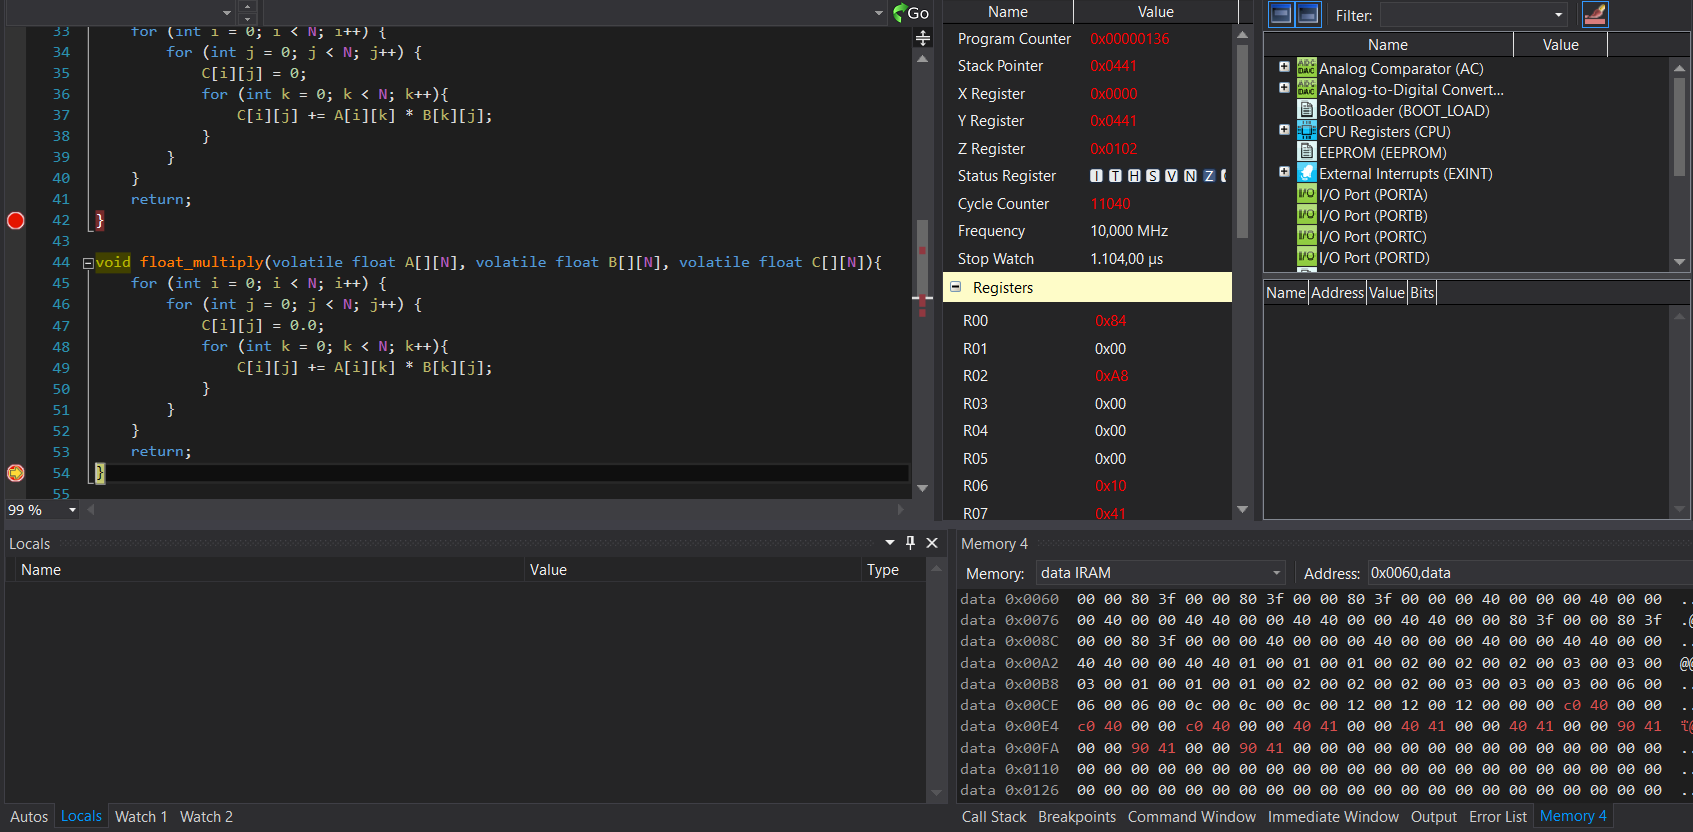
\includegraphics[height=3.5cm, width=\linewidth]{./results/lab10_sim_floats_b.png}
		\end{subfigure}
		\caption{Results from Αtmel Studio 7 - FLOAT multiplication}
	\end{figure}

	\noindent
	Όπως φαίνεται και στις παραπάνω προσομοιώσεις οι πόροι που χρησιμοποιεί το AVR είναι η μνήμη που διαβάζει τους πίνακες που πολλαπλάσιάζουμε και αποθηκεύει τα δεδομένα του αποτελέσματος, καθώς και κάποιοι καταχωρητές, για να κάνει τον πολλαπλασιασμό και το άθροισμα των αριθμών. Τέλος, παρατηρούμε ότι στον μικροελεγκτή AVR το γινόμενο integer 3x3 πινάκων χρειάζεται εμφανώς λιγότερους κύκλους σε σχέση με την περίπτωση που οι πίνακες που πολλαπλασιάζουμε είναι τύπου float. 
\end{document}
